\documentclass[12pt]{article}


%
% Packages
%

\usepackage{etoolbox}
\usepackage[capposition=top]{floatrow}
\usepackage{graphicx}
%\usepackage{caption}
%\usepackage{subcaption}
\usepackage{placeins}
\usepackage{setspace}
\usepackage{array}
\usepackage{fullpage}
%\usepackage[margin=1.5in]{geometry}
\usepackage{hyperref}
\usepackage{natbib}
\usepackage{microtype}
\usepackage{rotating}
\usepackage{amsmath}
\usepackage{morefloats}
\usepackage{float}
\usepackage{caption}
\usepackage{xcolor}
\usepackage[T1]{fontenc}
\usepackage[utf8]{inputenc}
\usepackage{authblk}
\usepackage{lmodern}

\hypersetup{
    colorlinks,
    linkcolor={black},
    citecolor={black},
    urlcolor={blue}
}
\usepackage{color,colortbl}
\usepackage{geometry}

\newcommand{\red}{\color{red}}
\newcommand{\blue}{\color{blue}}
\newtoggle{final}
%\togglefalse{final}
\toggletrue{final}


%
% Some utilities
%
%\usepackage{todonotes} % doesn't work - tikz lib too old
% define a mc=margincomment command
\iftoggle{final}{
   \newcommand{\mc}[2]{#1} % make margincomments go away
   \newcommand{\tc}[2]{#1} % make text comments go away
}%else
{
   \newcommand{\mc}[2]{% 1 referenced text 2 initials 3 comment
       \textcolor{blue}{#1}
       \marginpar{\scriptsize\textbf\raggedright\textcolor{red}{#2}}}
  \newcommand{\tc}[2]{\textcolor{blue}{#1}[\textcolor{red}{#2}]}
}

%
% Layout
%
\iftoggle{final}{
  \geometry{left=1.0in,right=1.0in,top=1.0in,bottom=1.0in}
}%else
{
  \geometry{left=0.5in,right=2.0in,top=1.0in,bottom=1.0in,marginparwidth=1.5in}
  }


\begin{document}

\title{Driving Past Commuting Zones: Re-examining Local Labor Market Definitions\thanks{Any opinions and conclusions expressed herein are those of the author(s) and do not necessarily represent the views of the U.S. Census Bureau. All results have been reviewed to ensure that no confidential information is disclosed, and no confidential data was used in this paper. This document is released to inform interested parties of ongoing research and to encourage discussion of work in progress.}}
\author[1]{Andrew Foote}
\author[1]{Mark Kutzbach}
\author[1,2]{Lars Vilhuber}
\affil[1]{Center for Economic Studies, U.S. Census Bureau}
\affil[2]{Labor Dynamics Institute, Cornell University}
\maketitle


\textbf{[Preliminary Draft - Do not cite without authors' permission]}


\begin{abstract}
This paper evaluates the suitability of local labor market definitions for representing the theoretical and empirical goal of assigning workers to distinct loci of commuting, wages, and employment opportunities. First, we revisit the commuting zone definitions from \citet{TS1996}. We discuss their methodology, highlighting two main weaknesses that affect the resulting labor market definitions. We then demonstrate how these weaknesses affect empirical estimates from a prominent paper using commuting zones. Finally, we define an objective function to measure the degree of integration in local labor markets and maximize it over an alternative clustering method. We conclude by comparing our method to other candidate local labor market definitions in the literature, and show that it is competitive with these definitions.
\end{abstract}


\doublespacing

%%%%%%%%%%%%%%%%%%%%%%%%%%%%
\section{Introduction}

Local labor markets are an important unit of analysis in labor economics, both in the theoretical and empirical literatures. Theoretical papers emphasize characteristics of a local labor market including common wage and rent levels \citep{Roback1982,Moretti2011}, as well as job-finding and unemployment rates \citep{HL2012,SS2014}.

In empirical labor economics, researchers may be interested in estimating the effect of some local, exogenous shock on labor market outcomes, and an important decision in any research design is defining the area that is directly affected by the shock. In estimating this effect, researchers have a number of different definitions of local labor markets from which to choose. \citet{BK1992}, \citet{Wozniak2010}, and \citet{KW2011} use the state, while other researchers use metropolitan areas \citep{BH2000,Card2001,Notowidigdo2011,Diamond2016}, while still others use counties \citep{MRR2015,FGS2015}.

One alternative labor market definition is commuting zones, which were originally defined by \citet{TS1996} (henceforth, TS1996). Commuting zones have two distinct advantages over the above definitions. First, they span the entire United States, allowing researchers to measure effects for the entire country rather than just metropolitan areas. Second, commuting zones group together counties based on commuting flows, which implies some level of economic integration (metropolitan areas are also based on commuting flows). The definition acknowledges that labor markets are not constrained by county and state lines, but are based on relevant linkages between counties.

Given these advantages, commuting zones have been used in a number of influential papers in the labor economics literature, including \citet{ADH2013}, as well as \citet{Yagan2016}, \citet{Restrepo2015} and \citet{AM2015}. Despite their widespread use, to the best of our knowledge, the methodology underlying commuting zone definitions and its impact on empirical estimates has not received much scrutiny. 

Our paper makes three contributions to the literature on local labor markets. First, we outline a number of methodological issues that researchers should be aware of when they use the commuting zone definitions. Second, we show how these methodological issues impact empirical estimates. Our findings suggest that researchers should consider evaluating the sensitivity of results to local labor market definitions. We propose two main ways that researchers can test to see if their results are robust to the uncertainty induced by commuting zones. Finally, we propose an alternative method similar to the one employed by Tolbert and Sizer, which allows us to measure integration beyond just commuting flows. We define a metric for the quality of a regionalization definition, and show that our proposed method performs better than alternative methods.

The remainder of the paper proceeds as follows. We describe the data we use in Section \ref{sec:data}, and then in Section \ref{sec:definitions} describes the commuting zone definition and methodology in detail. In Section \ref{sec:issues}, we discuss a number of issues with the commuting zone methodology. In Section \ref{sec:adhreplication}, we demonstrate how these issues impact empirical estimates. Finally, in Sections \ref{sec:objfn} and \ref{sec:ourmeth}, we discuss our measure of local labor market integration and methodology for defining local labor markets. Section \ref{sec:conclusion} summarizes and discusses next steps. 




%%%%%%%%%%%%%%%%%%%%%%%%%%%%%%%%%


\section{Data \label{sec:data}}

The primary data set that we use is the 1990 Journey to Work (JTW) data, which is derived from the 1990 Census long form. In the JTW questions, employed respondents are asked ``at what location did this person work LAST WEEK (If this person worked at more than one location, print where he or she worked most last week.'' The 1990 JTW data geocodes these responses and publishes estimated home-to-work flows for all counties and county equivalents in the United States.\footnote{This data, as well as the ACS data described later, is available for download from the Census website, at \url{http://www.census.gov/hhes/commuting/data/commutingflows.html}} The Office of Management and Budget (OMB) uses JTW in its guidelines for defining Metropolitan Statistical Areas, a geographic unit used for research, statistical publications, and federal programs.\footnote{See the Federal Register Part IX, Office of Management and Budget: Standards for Defining Metropolitan and Micropolitan Statistical Areas; Notice, December 27, 2000, available  at \url{http://www.census.gov/population/metro/files/00-32997.pdf}} \citet{TS1996} use the 1990 JTW data for their analysis. We use the 1990 JTW data to replicate TS1996's Commuting Zone definitions, as well as estimate our alternate labor market definitions. 

In addition to the 1990 JTW data, we also use the 2000 JTW data, and the 2009-2013 5-Year Pooled American Community Survey JTW data. The ACS data are similar to the Decennial Census data, but include fewer pairs of counties in the published flows data. The JTW from ACS also includes published margins of error for these flows, whereas the 1990  and 2000 JTW data do not include these measures.

Table \ref{tab:comstat} provides summary statistics on the worker flows data from the three main data sources. We summarize the number of residence counties in the file, the total count of jobs included in the flows, the mean residence labor force and home-to-work flow sizes, and the mean share of workers who work in the same county where  they live. We note the rise in population, or total job count, from 1990 through 2009, as well as the declining share of within-county commuting during that period (a lower within-county share). The decline in the share of within-county commuting, which shows an increased distance of jobs from where workers live, is consistent both with studies of Census and ACS data showing increasing travel time in recent years \citep{ACS2011}. 

We use a number of other data sources to measure local labor market integration in Section \ref{sec:objfn}: county-level unemployment rates from the Bureau of Labor Statistics Local Area Unemployment Statistics series; and annual earnings data from the Bureau of Economic Affairs Regional Economic Indicators Series (REIS), both from 1990-1995, which aligns most closely with the timing of our commuting data.

% table cluster changes
\begin{table}\centering
\caption{Commuting Summary Statistics \label{tab:comstat}}
\begin{tabular}{lccccc}
\hline\hline
 & & Total & Mean & Mean & Mean \\ 
 & & Residential & Residential & Flows & Within-county \\ 
Dataset & Counties & Labor Force & Labor Force & Home-to-work & Share of Flows \\ 
\hline
\multicolumn{6}{l}{\emph{Journey-to-Work (JTW) Estimates}}\\
1990 Census & 3,105 &   115,004,732 & 460,966 & 392,408 & 0.76 \\ 
2000 Census & 3,107 &   128,170,381 & 444,149 & 369,102 & 0.74 \\ 
2009-2013 ACS & 3,143 & 139,679,674 & 505,765 & 419,784 & 0.73 \\ 
%\hline
%\multicolumn{6}{l}{\emph{LODES Data}}\\
%2006 & 3,125 &        124,088,835 & 460,908 & 335,992 & 0.60 \\ 
%2007 & 3,125 &        125,922,964 & 459,064 & 329,053 & 0.58 \\ 
%2008 & 3,125 &        126,100,097 & 463,321 & 330,606 & 0.57 \\ 
%2009 & 3,121 &        121,594,710 & 441,584 & 312,014 & 0.56 \\ 
%2010 & 3,126 &        123,193,014 & 445,503 & 313,439 & 0.56 \\ 
%2011 & 3,126 &        125,903,901 & 452,765 & 318,870 & 0.55 \\ 
%2012 & 3,022 &        125,554,526 & 456,308 & 321,988 & 0.55 \\ 

\hline
\multicolumn{6}{p{6in}}{\footnotesize \textit{Notes}: Authors' calculations, using public-use county-to-county flows from Journey to Work estimates for the 1990 Census, 2000 Census, and the 2009-2013 5-Year ACS.}\\
\end{tabular}
\end{table}



%%%%%%%%%%%%%%%%%%%%%%%%%%%%%%%%%%%%%%%%%%%

\section{Commuting Zone Methodology \label{sec:definitions}}

\subsection{Background}

As an alternative to metropolitan statistical areas (or Core Based Statistical Areas), many researchers use Commuting Zones because they cover the entire country and group counties based on commuting flows, which is a measure of labor market integration. However, few researchers are familiar with the underlying methodology. To that end, this section describes the commuting zone  methodology, as developed by TS1996. 

The methodology was  originally developed in \citet{TK1987}, but the 1996 paper is much more widely cited. The Economic Research Service (ERS), an agency under the Department of Agriculture for which this methodology was developed, distributes commuting zone definitions on its website. Commuting Zones are especially relevant for the economic analysis of rural areas because the include all counties, not just urban counties. ERS also distributes a version of Commuting Zones based on 2000 data. For a research into extending the time series of Commuting Zones and further background on TS1996, see \cite{FowlerRhubartJensen2016}.

To define an exhaustive classification of counties, TS1996 calculated a dissimilarity matrix $D$, where an entry $D_{ij}$ is the dissimilarity of county $i$ from county $j$, calculated as below:\footnote{Due to computational constraints at the time, TS1996 broke the country into six overlapping regions: Northeast, Southeast, Midwest, Southwest, Central and West, calculating a separate distance matrix for each region.}
\begin{equation}\label{eqn:distance}
D_{ij} = 1- P_{ij} = 1- \frac{f_{ij} + f_{ji}}{\min(rlf_i,rlf_j)}
\end{equation}
where $f_{ij}$ is the number of commuters who live in $i$ and work in $j$, and $rlf_i = \sum_{j} f_{ij}$ (including $f_{ii}$) is the resident workforce. The data used in TS1996 to estimate the flows is from the \mc{1990 Journey to Work data}{LV: Reference/bibliographic entry}, released from the 1990 Census. Other releases based on data from the 1980 and 2000 Censuses are also available.\footnote{These CZ definitions are available at \url{http://www.ers.usda.gov/data-products/commuting-zones-and-labor-market-areas.aspx}}
After constructing this dissimilarity matrix, they use it as the input into an average-linkage hierarchical clustering algorithm (\mc{PROC CLUSTER in SAS}{LV: Cite the online PDF explaining the procedure for SAS 9.2, see if you can find the proper quote for SAS 6.12, which was likely the version they used - might be in the Census library, or even in LEHD}). They allow clusters to form that are no higher than a `height' of 0.98.\footnote{In the average-linkage clustering algorithm, the height (or distance) between clusters is given by the following formula:
\[
D_{KL} = \frac{1}{N_K N_L} \sum_{i \in C_k} \sum_{j \in C_L} d(x_i,x_j)
\]
That is, the distance between two clusters is the average of the pair-wise distances between each component of the two clusters. Therefore, that implies no clusters were merged such that $D_{KL}>0.98$.  (\href{https://support.sas.com/documentation/cdl/en/statug/63347/HTML/default/viewer.htm\#cluster_toc.htm}{SAS Manual, version 9.2})} Additionally, because they cluster separately for region, and there are a number of states that are in multiple regions, they manually reconcile these competing cluster definitions, but do not provide their methodology for this reconciliation in the paper. Finally, they mention that they do perform a national analysis, but do not report the results.

We illustrate the process in Appendix Figure \ref{fig:caliclusters}, which shows how the counties are clustered together for California. In the top left-hand corner, only a few counties have joined at a height of 0.8. As we increase the height of allowable clusters from 0.8 to 0.88, more counties are joined together to make clusters, and the same is true when increasing the height to 0.96. Finally, at a height of 1, almost all the counties have merged together and there is one large cluster and a few much smaller clusters.

\subsection{Replicating Tolbert and Sizer's Definitions}

% Source program: /modules/module_mapjtw1990.sas
% Last updated:


%%%%% COMMUTING ZONES
\begin{figure}[th]
\caption{Replication of Commuting Zones from TS1996: County Mapping}
%\begin{subfigure}[t]{0.5\textwidth}
\begin{tabular}{cc}
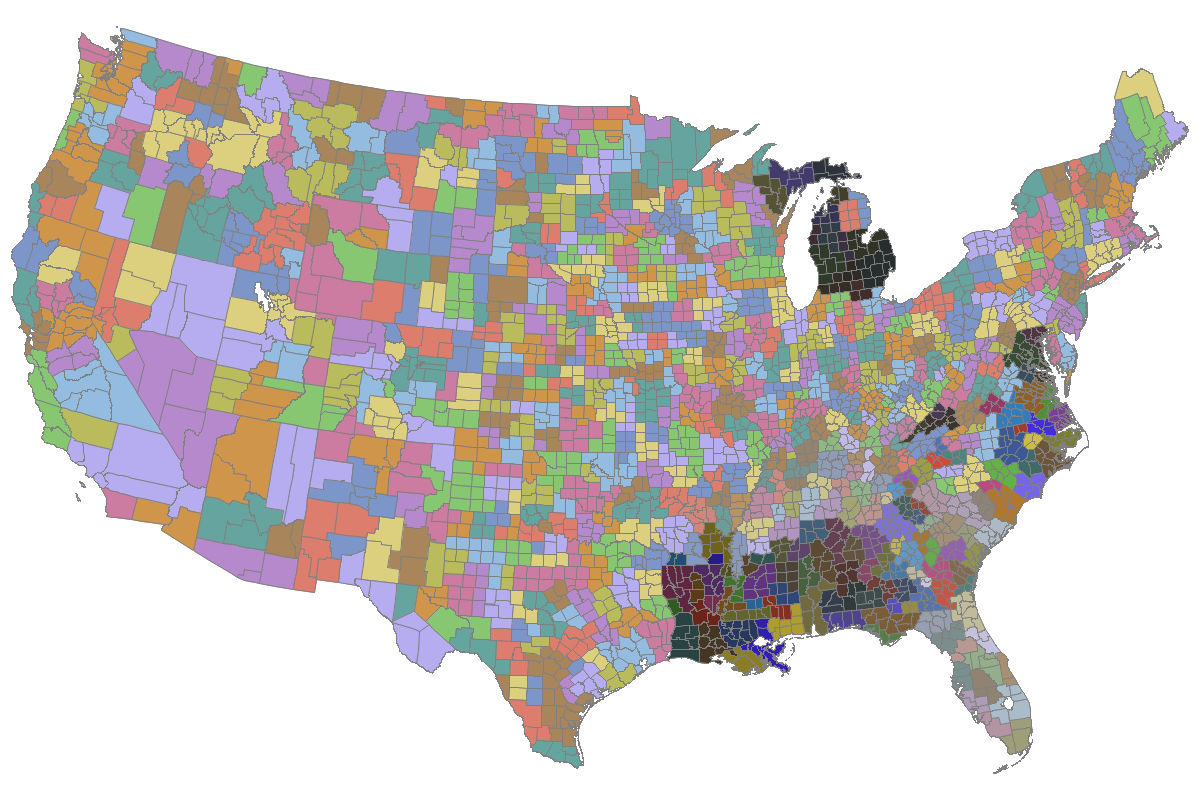
\includegraphics[width=.48\textwidth]{./figures/commutingzones.png}
&
%\caption{Tolbert and Sizer's Commuting Zones}
%\end{subfigure}
%\begin{subfigure}[t]{0.5\textwidth}
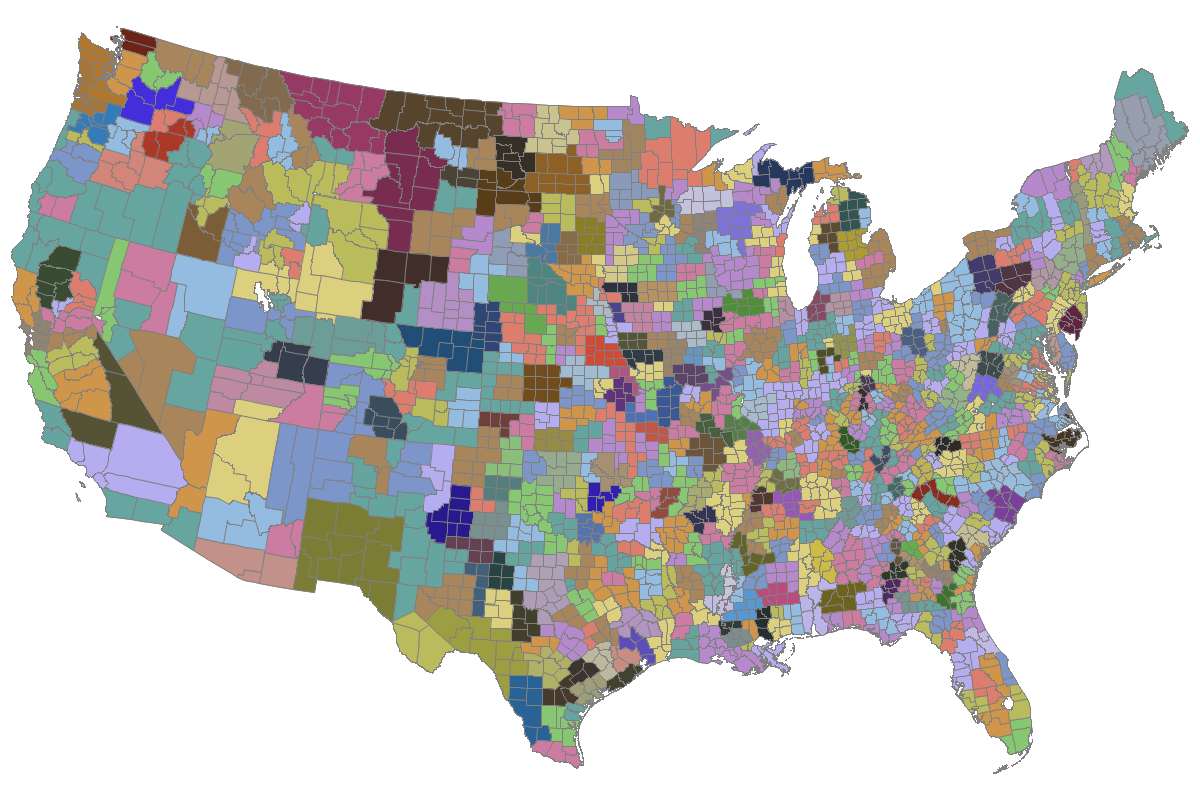
\includegraphics[width=.48\textwidth]{./figures/replication.png}
\\
{Commuting Zones from TS1996: TS1990}
&
{Replication of Commuting Zones: FKV1990}
\\
\end{tabular}
\label{fig:czmaps}
\end{figure}


% source: name of SAS program
% Last updated:

\begin{table}\centering
\caption{Replication of Commuting Zones from TS1996: Summary Statistics \label{tab:replication}}
\begin{tabular}{lcc}
\hline\hline
       & TS1990 &  FKV1990  \\
       \hline
Mean Cluster Size &  4.24  & 4.19 \\
Median Cluster Size & 4 & 4 \\
Number of Clusters & 741 & 741  \\
Number of Singletons & 62 &  10 \\
\hline
\multicolumn{3}{p{4in}}{\footnotesize \textit{Notes}: Both TS1990 and FKV1990 are based on JTW tabulations from the 1990 Census. Summary statistics for TS1990 are from Table 8 of TS1996.}\\
\end{tabular}
\end{table}



In order to replicate the clustering result in TS1996, which we refer to as TS1990, we use the 1990 Census JTW data and the methodology described above.\footnote{Rather than splitting the country into separate regions, we perform our clustering at the national level, because it is computationally feasible to do so. We attempted to replicate their methodology at the regional level, but were unable to determine how they reconciled competing definitions across regions. \cite{FowlerRhubartJensen2016} document the expert review process in the original Commuting Zone delineations.} 
Our analysis showed that using a height cutoff of 0.9418 gives us results that are closest to the TS1990 mapping. We refer to the resulting clusters as FKV1990. Figure \ref{fig:czmaps} shows a visual comparison of TS1990 and FKV1990 communting zones, while Table \ref{tab:replication} shows summary statistics of TS1990 and FKV1990. There are 739 clusters in FKV1990, compared with  741 clusters in TS1990. In both sets, the average number of counties per cluster is 4.24, while the median is 4.

We also calculate two similarity measures between the clusters: for each county, the share of counties in our clusters that are in the same TS1990 commuting zone; and the share of counties in a TS1990 commuting zone are in the same cluster (unweighted). Both metrics are  over 80\%. Overall, we conclude that while not exactly identical, the FKV1990 replication of TS1990 is reasonably close.\mc{}{MK: Are these job weighted?}



%%%%%%%%%%%%%%%%%%%%%%%%%%%%%%%%%%%%%%%%%%%%

\section{Sensitivity Analysis of the Commuting Zone Methodology \label{sec:issues}}

While Commuting Zones are thought of as representing local labor markets, they have a number of shortcomings for empirical research that are not regularly discussed in the literature. In this section, we evaluate the sensitivity of Commuting Zone definitions for two aspects of the TS1996 methodology. First, the method is highly sensitive to variation in the input data, and if the input data are measured with error, the definitions may convey a false sense of certainty. Second, the resulting clusters are very sensitive to the decision of when to stop merging clusters, which implies that small changes in the chosen cutoff height drastically affect the number and size of clusters. Overall, this uncertainty in the definition of commuting zones contributes to conventional standard errors understating the true level of uncertainty in estimates, as well as non-classical measurement error that may bias empirical estimates. At the end of the section, we list other weaknesses that also undermine commuting zones as a definition of local labor markets.

\subsection{Sensitivity of Clustering Results to Underlying Error}
Given the reliance of TS1996 on the commuting flows data, we want to analyze the extent to which the outputs of the TS1996 methodology are sensitive to error in the input data. First, recall equation \ref{eqn:distance} for the dissimilarity matrix entries. If $f_{ij}$ is measured without error, then $D_{ij}$ is measured without error. However, if the flows are measure with some error, $\epsilon_{ij}$, then we have an estimate of $D_{ij}$, $\hat{D}_{ij}$, which can be expressed as below:
\begin{equation}
\hat{D}_{ij} = 1- \hat{P}_{ij} = 1- \frac{f_{ij}+\epsilon_{ij} + f_{ji} + \epsilon_{ji}}{\min(\hat{rlf}_i,\hat{rlf}_j)}
\end{equation}	
Now suppose without loss of generality that county $i$ is the smaller county; that means that 
\[
\hat{D}_{ij} =1- \frac{f_{ij}+\epsilon_{ij} + f_{ji} + \epsilon_{ji}}{ rlf_i + \sum_j \epsilon_{ij}}
\]
Or, rewritten:
\[
\hat{D}_{ij} =1- \frac{f_{ij} + f_{ji} }{rlf_i + \sum_j \epsilon_{ij}}+\frac{\epsilon_{ij} + \epsilon_{ji}}{ rlf_i + \sum_j \epsilon_{ij}}
\]
However, even if $E[\sum_j \epsilon_{ij}]=0$, we only have one realization of this draw (the published figures), which were calculated from survey responses. Additionally, we know two things about $\epsilon_{ij}$. First, $\epsilon_{ij} / f_{ij}$ is larger for smaller counties. Second, this implies that $rlf_i$ is 
more subject to measurement error for small counties than larger counties.
This will increase $D_{ij}$ for some small counties and decrease it for others. Because of the hierarchical nature of the clustering method, this will affect the formation of all other clusters in the data.\footnote{Additionally, because the heights are normalized in the procedure, it also affects where the effective cutoff is, even for counties unaffected by errors in flows.}

To demonstrate how this measurement error affects the outcome of the clustering procedure, we use journey-to-work data from the pooled 2009-2013 ACS because it has published margins of error (hereafter, MOEs).\footnote{In the 2009-2013 ACS, the average ratio of margin of error to reported commuting flow (unweighted) is 1.24. The Decennial Census numbers do not publish margins of error, but presumably they are somewhat smaller than ACS MOEs. Later in the paper, we use the 2009-2013 ACS MOEs to estimate the MOEs for the 1990 JTW flows.} For reference, summary statistics on the ratio of the margins of error to the flows are in Table \ref{tab:moesum} in the appendix, and show that margins of error are much larger relative to smaller flows. Using these MOEs, we perform the following analysis: 

\begin{enumerate}
	\item For each origin-destination pair, we draw $\epsilon_{ij}$ from a normal distribution
 with mean 0 and standard deviation $MOE_{ij}/(2 \times 1.64)$, since the MOE is the 90\% confidence interval.
	\item Add the value from (1) to the reported flow ($\hat{f}_{ij} = f_{ij} + \epsilon_{ij}$).
	\item Re-aggregate the flows, recalculate the dissimilarity matrix, and re-run the TS1996 clustering procedure.
	\item Using the new clusters, calculate the following statistics: average number of counties in a cluster; the number of clusters; and the total number of counties in a different cluster than the one they would have been assigned, had the flows been assigned using only the published flow estimates (that is, not taking into account the MOE).
\end{enumerate}
%
% Source program: module_perturbjtw2009.sas
% Last updated:

\begin{figure}[th]
\caption{Sensitivity Analysis}
%\begin{subfigure}
\begin{tabular}{ccc}
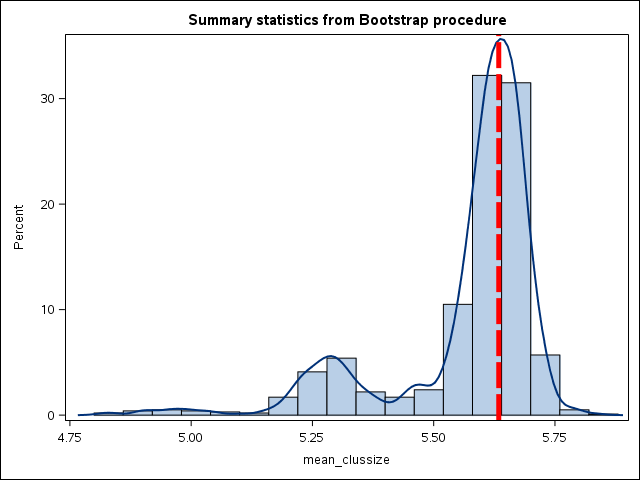
\includegraphics[width=0.33\textwidth]{./figures/mean_clussize_jtw2009.png}
&
%\caption{Mean Cluster Size}
%\end{subfigure}
%\begin{subfigure}
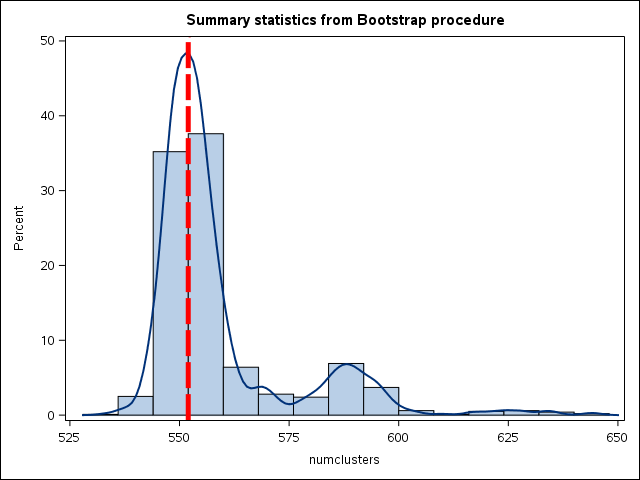
\includegraphics[width=0.33\textwidth]{./figures/numclusters_jtw2009.png}
&
%\caption{Number of Clusters}
%\end{subfigure}
%\begin{subfigure}
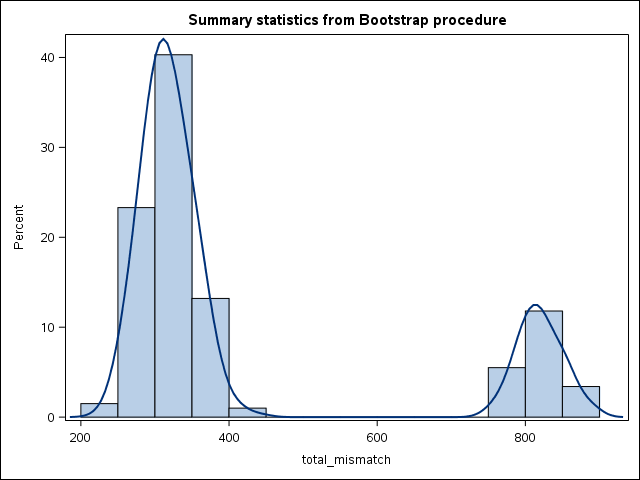
\includegraphics[width=0.33\textwidth]{./figures/mismatchedcounties_jtw2009.png}
\\
{(a) Mean Cluster Size}&
{(b) Number of Clusters}&
%\caption
{(c)Mismatched Counties}
\\
\multicolumn{3}{p{6.2in}}{\footnotesize \emph{Notes:} Histograms plot the density of summary statistics from commuting zones produced using the TS1996 methodology from 1000 simulations of Margins of Error from the 2009-2013 ACS commuting flows data. Red lines provide the summary statistics from commuting zones produced from the published ACS estimates (mean cluster size of 5.63 for 552 clusters).}\\
%\end{subfigure}
\end{tabular}
\label{fig:perturbation}
\end{figure}
\normalsize 


%
We iterate over this procedure 1000 times in order to obtain distributions for these statistics. These graphs are shown in Figure~\ref{fig:perturbation}, where the red vertical dashed lines are the values that would be obtained using only the published figures (without MOE purturbations). Note that there are fewer clusters in the TS1996 implementation for JTW based on ACS, with 551 formed based on the published data compared with 741 in TS1990 and 709 in TS2000.\footnote{We use the same cutoff here as in FKV1990, our replication of TS1990. While commuting flows have increased in distance since 1990 (see Table \ref{tab:comstat}), it is not clear why the same methodology on later data results in so many fewer zones. These results hold irrespective of cluster height.} As one can see, the average cluster size has a wide range of values; while most values are around what the published numbers would give, there is still a substantial portion that have smaller than average clusters. Second, the number of clusters ranges widely, 330 to 450. Finally, the share of population that is mismatched is on average about 5\% of the US population, a small but non-negligible number.
Overall, the underlying measurement error in the data causes uncertainty in the cluster definitions, which is exacerbated by the sharp cutoff imposed in cluster analysis, which we discuss in the next subsection.

\subsection{Distribution of Cluster Height \label{sec:clusterheight}}

We turn to the sensitivty of the clustering to the chosen cutoff value. \citet{TK1987}, describe the algorithm for choosing a cutoff value as follows: ``As a rule of thumb, a normalized average distance of 0.98 was considered sufficient distance between sets of counties to treat them as separate [Labor Market Areas]'' \citep[page 15]{TK1987}.  The article does not provide an analysis of the sensitivity to changing the cutoff marginally up or down. In this subsection, we investigate how sensitive the resultant clusters are to the choice of the cutoff value.


% Source program: /modules/module_clustjtw1990.sas
% Last updated:


%%%%% COMMUTING ZONES
\begin{figure}[th]\centering
\caption{Distribution of Cluster Consolidation, by Height }
\begin{tabular}{c}
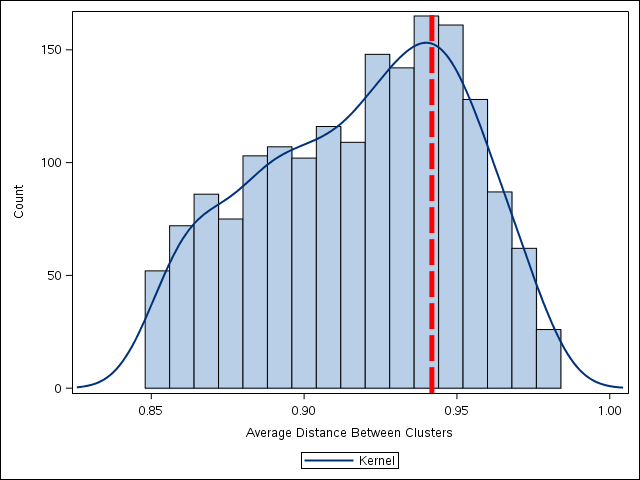
\includegraphics[width=.48\textwidth]{./figures/distancebetweenclusters.png}\\
\multicolumn{1}{p{4in}}{\footnotesize \emph{Notes:} Histograms plot number of
clusters that form at various heights, based on hierarchical clustering
procedure. The vertical line is the value that most closely replicates TS1990.}
\label{fig:heightdensity}
\end{tabular}
\end{figure}



Figure \ref{fig:heightdensity}  show the distribution of heights at which clusters merge using the national 1990 JTW data, with the vertical line indicating the cutoff we chose that most closely approximated TS1996 (0.9418). The key takeaway from this figure is that marginally increasing or decreasing the cutoff causes a substantial number of clusters to be formed or not. In fact, increasing the cutoff to 0.9428 causes the number of clusters to fall by 19, while decreasing the cutoff to 0.9408 causes the number of clusters to increase by 17.\footnote{Another consideration, not discussed here, is that TS1996 normalize the heights within each region before clustering. This causes the cutoff to be at different absolut heights depending on the region.}

As we described above, the measurement error in commuting flows causes some uncertainty in terms of true dissimilarity, and hence true cluster height. Because of the presence of a strict cutoff, some clusters that would have formed (if there were no measurement error) did not form, and vice-versa. More broadly, TS1996 provide no empirical guidance for choosing the `optimal' cutoff and cluster size other than referring to expert knowledge. Later, in Section \ref{sec:objfn}, we consider measures of local labor market integration that may be informative of the optimality of various clustering definitions. 

%\subsection{Other Weaknesses of CZ Methodology}

%In addition to the uncertainty due to data and methodology detailed above, commuting zone construction has a few other features that make it a less than ideal description of local labor markets. First, because the method does not consider the size of counties, the commuting zones in the East half of the country are systematically smaller than the zones on the West half of the country, solely because of the size of the counties. Second, because commuting zones are defined solely based on commuting flows, they do not fully capture local labor market integration; as we noted earlier, these only capture \textit{realized} flows at a point in time, not historical or potential flows. Finally, the clustering method used in TS1996 is very dependent on the order of the first few clusters formed, which makes it more sensitive to error in the data inputs than other clustering methods.	

%First, if we define local labor markets only based on \emph{realized} commuting flows, we overlook other ways in which labor markets are integrated, such as wage levels and unemployment rates. Second, solely using commuting flows is also an issue because they are measured using survey data, and hence are subject to sampling error. This second fact, paired with the strict cutoff, overstates the certainty in the commuting zone defintions.



%%%%%%%%%%%%%%%%%%%%%%%%%%%%%%%%%%%%%%%%%%%%%%

\section{Robustness of Empirical Estimates to Commuting Zone Uncertainty \label{sec:adhreplication}}

While we have shown that commuting zone definitions are sensitive to input data and parameters, this sensitivity only matters insofar as it impacts empirical estimates. We demonstrate the consequences of this sensitivity using a well know example of estimates measured at the commuting zone level.

In their paper, \citet{ADH2013} estimate the impact that increased trade competition from China had on manufacturing employment in the United States. To estimate this effect empirically, they use variation in the initial distribution of manufacturing employment at the commuting zone level and national increases in imports from China by manufacturing subsector. Because they use commuting zones as their definition of the local labor market, their empirical analysis is exposed to the critiques we have discussed above.\footnote{We want to acknowledge that Autor, Dorn and Hanson have been incredibly helpful in the process of replicating their paper, both in providing data and helping troubleshoot, as well as being receptive to this exercise.}

Their main estimating equation in the paper is as follows:

\begin{equation}\label{eqn:adh}
\Delta L_{it}^m = \gamma_t + \beta_1 \Delta IPW_{uit} + \beta_2 X_{it} + e_{it}
\end{equation}

Where $\Delta L_{it}^m$ is the decadal change in manufacturing employment in Commuting Zone $i$ following year $t$, $\Delta IPW_{uit}$ is the import exposure measure for the United States, and $X_{it}$ are control variables. All regressions are weighted by population share of the commuting zone.

Since we use slightly different methods of aggregating data, we compare the main estimates from \citet{ADH2013} (Table 1 in their paper) to our replication, which we show in Table \ref{tab:adhreplication}. Each cell in the table is a coefficient from a different regression, and for simplicity we just estimate it for the time period 1990-2000 (other results available upon request). The first column shows the estimates from their paper, while the second column changes the import exposure measures to our replicated measure. In the third column, we use our estimate of the change in manufacturing employment amd weights, rather than the estimate and weights from their data. The final column clusters on commuting zone rather than state.

Overall, the estimates are considerably stable, giving us confidence that we are properly replicating their initial findings. We now turn to demonstrating how these estimates are affected by the concerns with the commuting zone definitions themselves.


% source: name of SAS program
% Last updated:

\begin{table}\centering
\caption{China Syndrome Replication and Comparison, 1990-2000 \label{tab:adhreplication}}
\begin{tabular}{lcccc}
\hline\hline
       & ADH Estimate & Our RHS & Our LHS and Weight & CZ Clustering  \\
       \hline
$\Delta IPW_{cz,t}$ & -0.8875 & -0.8871 & -0.8748 & -0.8748 \\
                   & (0.1812) & (0.1811) & (0.1527) & (0.1243) \\

\hline
\multicolumn{5}{p{6in}}{\footnotesize \textit{Notes}: Table from author's calculations, using data from \citet{ADH2013} and constructed data, based on equation \ref{eqn:adh}. Column 1 is Table 2, Column 1 from ADH (2013). Column 2 replaces their measure of import exposure to ours. Column 3 replaces their measure of change in manufacturing employment and CZ-specific weights with ours. Column 4 does not cluster on state. Standard errors are in parentheses. All coefficients are significant with p-values less than 0.01.}\\
\end{tabular}
\end{table}



\subsection{Effect of Errors in Flows Data}
\FloatBarrier

First, we show how the estimate is affected based on MOE in the commuting flows input data. For this exercise, we used the distribution of margins of error published in the 2009-2013 ACS flows, and matched the ratio based on the flow sizes of the 1990 JTW data.\footnote{These flow size bins are the following percentile bins: 0-50; 50-90; 90-95; 95-99; and 99+.} We then draw from a normal distribution implied by the margins of error, and calculated a new dissimilarity matrix with the perturbed  flows. Using the same cutoff that we used for our replication of TS1996, we produce a new realization of commuting zones, and then repeat the above procedure 1000 times.

\begin{figure}\centering
\caption{Distribution of Effect, 1990-2000 \label{fig:1990dist}}
\begin{tabular}{c}
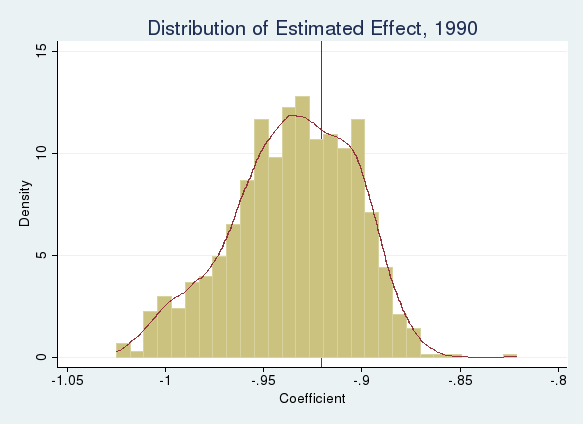
\includegraphics[scale=.5]{./figures/1990_distribution.png}\\
\multicolumn{1}{p{4.5in}}{\footnotesize \emph{Note:} Histogram plots estimates of $\beta_1$ from equation \ref{eqn:adh}, based on commuting zone realizations as outlined in Section \ref{sec:issues}.}
\end{tabular}
\end{figure}

We use these different commuting zone definitions to aggregate counties and then estimate equation \ref{eqn:adh}. These estimates are graphed in Figure \ref{fig:1990dist}, which shows the distribution of the estimated effect for the 1990-2000 period, and the red vertical line shows the estimate under the standard commuting zone defintions. The estimates are somewhat dispersed, with the left tail of the distribution almost 10\% lower than the estimate from ADH; however, the values are within two standard errors of the original estimate. Additionally, the distribution is skewed to the right.

This exercise demonstrates that there is additional uncertainty induced by the construction of the commuting zones that is not addressed in empirical estimates that use these definitions, which may overstate the precision of the results.

%Overall, this underscores the considerable uncertainty in commuting zones, and how this affects empirical estimates in one way. However, there is also ambiguity in how the commuting zones are constructed for reasons separate to the flows. For this discussion we turn to the next subsection.

\subsection{Effects on the Chosen Cutoff}

\begin{figure}\centering
\caption{Differences in Effect Based on Cluster Cutoff \label{fig:cutoff_dist}}
\begin{tabular}{cc}

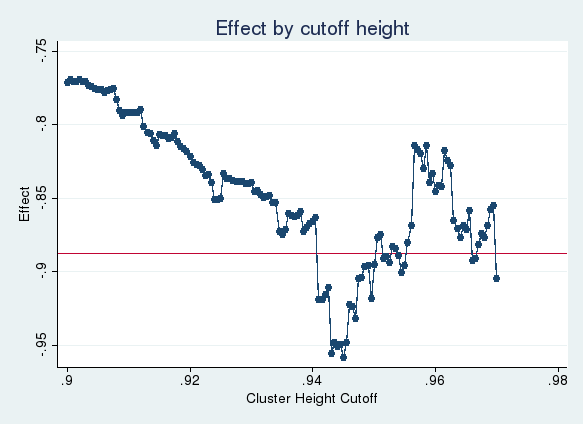
\includegraphics[scale=.4]{./figures/cutoff_1990.png} & 
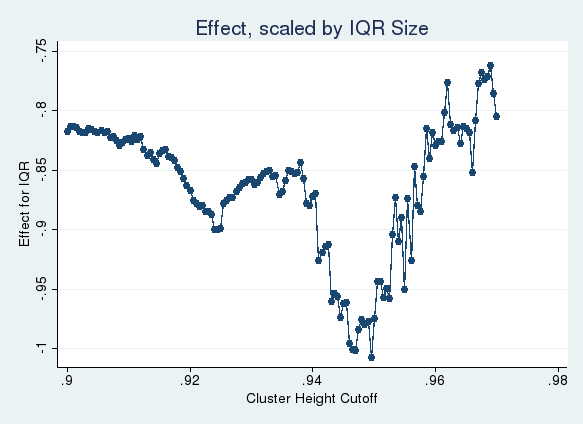
\includegraphics[scale=.4]{./figures/cutoff_iqr_1990.png}\\
(a) Effect by Cutoff Height & (b) Effect by Cutoff Height, Scaled by IQR \\

\multicolumn{2}{p{6.5in}}{\footnotesize \emph{Note:} Author's calculations based on replication of Tolbert and Sizer's method. Panel (a) shows estimates of $\beta_1$ from equation \ref{eqn:adh} for different definitions of commuting zones based on height cutoff, while Panel (b) shows estimates of $\beta_1$ scaled by the difference in exposure between the 25th and 75th percentile commuting zone. The horizontal line in panel (a) is the main estimate from \citet{ADH2013}}
\end{tabular}
\end{figure}

In addition to the uncertainty that is induced by underlying error in the commuting flows, in Section \ref{sec:clusterheight} we showed that the decision of where to stop the clustering process was rather arbitrary, since there is no clear guidance on what cutoff is most appropriate. To demonstrate how the cutoff choice affects the estimate of $\beta_1$ from equation \ref{eqn:adh}, we generate clusters based on cutoffs between 0.9 and 0.97 and estimate the model using the resulting clusters.

Figure \ref{fig:cutoff_dist} displays the results of this exercise, where panel (a) shows the raw coefficient, and panel (b) shows the coefficient scaled by the interquartile range of $\Delta IPW_{uit}$, since this changes depending on the cutoff. In panel (a), the red horizontal line is the estimate from ADH.

Again, our results show that there is some variation in the estimate based on the cutoff value. Around the cutoff value that most closely replicates TS1996, the estimate is the most negative. However, cutoff values marginally higher or lower give different results, which reinforces the point we made with Figure \ref{fig:heightdensity} - the number of clusters that merge is incredibly dense near the cutoff for commuting zones, so that any change in the cutoff changes the commuting zone definitions non-neglibly. This density causes estimates using commuting zone observations to change near the cutoff. Given the sensitivity of estimates to the chosen cutoff, best practices would be to report estimates for a broad range of cutoffs.


%%%%%%%%%%%%%%%%%%%%%%%%%%%%%%%%%%%%%%%%%%%%%%

\section{Objective Function for Measuring Local Labor Market Integration \label{sec:objfn}}

Up to this point, we have focused on the commuting zone methodology exclusively. However, in the next two sections we turn to two important issues: how to measure labor market integration, and an alternative clustering method that does not have the drawbacks of the hierarchical technique.

The theoretical literature consistently defines a local labor market as characterized by similar wages, unemployment rates, and commuting links within the area. However, there are no established methods for measuring how appropriate a set of local labor markets is in approximating the theoretical area.

To that end, we formulate an objective function to evaluate how well any given local labor market definition reflects this theoretical construct. To be specific, we measure four statistics that reflect the integration of an area in terms of unemployment and wage series as well as in- and out- commuting rates.\footnote{We have considered additional measures that correspond to the theoretical literature, including housing or rental price series and compactness, which could be measured by average pairwise distance.} 

First, for both unemployment rate and wages (using BLS data), we measure the average pairwise correlations between counties in a cluster, which are $\bar{\rho}_i^{URATE}$ and $\bar{\rho}_i^{Wages}$, respectively.\footnote{The pair-wise correlations between counties are calculated using six years of data (for this paper, that is 1990-1995).
\[
\bar{\rho}_i^{URATE} = \frac{1}{2N} \sum_{i \in C} \sum_{j \in C} \rho_{i,j}
\]} The higher these values are, the more integrated the counties are.

Second, we measure commuting flows into the labor market from other counties, as a share of the local labor force, as well as commuting flows to outside areas ($InflowShare_i$ and $OutflowShare_i$). We expect that the commuting flows within a labor market ought to be much higher than commuting flows outside of the labor market, reflecting an integrated area, such that a higher value of these measure reflects lower labor market integration. We sum these measures across labor markets in the following manner:

\begin{equation}\label{eqn:objfn}
	Objfn(C) = \frac{1}{4N_c} \sum_{i\in C} (\gamma_1 \bar{\rho}^{URate}_i + \gamma_2 \bar{\rho}^{Wages}_i - \gamma_3 InflowShare_i - \gamma_4 OutflowShare_i )
\end{equation}

Where $Objfn(C)$ is the objective function value for a definition of local labor markets, $C$ The $\gamma$ factors are normalization weights, since $\bar{\rho}$ and the commuting shares are on different scales.\footnote{We normalize these values by taking random clusters of 5 counties and calculating each component of equation \ref{eqn:objfn}, then calculating the mean; in this exercise, the values of $\gamma$ are just the inverse of these means, although there may be other candidate weights.} Given that a larger objective function value reflects a more integrated local labor market, when comparing two competing definitions of local labor markets, the definition with the higher objective function value is the better labor market definition. More formally, for two local labor market definitions, $C$ and $D$, if $Objfn(C)>Objfn(D)$, then $C$ is the more appropriate local labor market.

In the next section, we develop a methodology using this objective function, such that our resulting local labor market definitions maximizes the objective function.

%\subsection{Benchmarking Objective Function Values}

%To have a benchmark to normalize objective function values, so that they are comparable over time, we propose using a ``worst-case'' local labor market. Specifically, we randomly group counties into sets of 5, irrespective of where they are in the country. These definitions should not reflect any labor market integration other than the underlying integration of the national labor market, which varies over time, and allows us to take out changes in the objective function over time based on overall dispersion of labor market conditions or time-varying quality of the available data.\footnote{In practice, this exercise is similar to adding year fixed-effects to a regression, in order to absorb variation that is common to the country as a whole in a given year. Because dispersion in unemployment and wages rates is different across years and business cycles nationally, some of the changes in $Objfn(C)$ reflect national-level phenomena rather than local labor market integration.}

%% table cluster changes
\begin{table}\centering
\caption{Summary Statistics of the Allocation of Counties to Clusters, by Local Labor Market Definition\label{tab:clustersum}}
\begin{tabular}{lccccccc}
\hline\hline
Cluster scheme & Clusters & Counties & Median & Mean & StdDev & Min & Max \\ 
\hline
Commuting Zones 1990 & 741 & 3,141 & 4 & 4.24 & 2.50 & 1 & 19 \\ 
Commuting Zones 2000 & 709 & 3,141 & 4 & 4.43 & 2.48 & 1 & 19 \\ 
CBSAs and State remainders & 962 &    3,142 &  1 & 3.2661 &  8.1104 &   1 &    126 \\ 
States & 51 & 3,142 & 62 & 61.61 & 46.76 & 1 & 254 \\ 
Randomized Zones & 621 & 3,105 & 5 & 5 & 0 & 5 & 5 \\ 
Mobility Zones & 512 & 3,108 & 6 & 6.07 & 2.34 & 1 & 14 \\ 
\hline
\multicolumn{8}{p{6.5in}}{\footnotesize \textit{Notes}: The definitions of 1990 and 2000 Commuting Zones are based on the TS1996 methodology and are the clusters provided by the Economic Research Service. CBSA mappings of counties are based on Office of Management and Budget definitions. Randomized Zones and Mobility Zones are Authors' calculations, with Mobility Zones using public-use tabulations of Journey to Work for the 1990 Census as well as the Local Area Unemployment Statistics from the Bureau of Labor Statistics and earnings data from Bureau of Economic Affairs.}\\
\end{tabular}
\end{table}



%These results are striking. We see that in 1990, the 1990 Commuting Zones have the lowest objective function values, while states and CBSAs have much higher values. But in 2000, the 1990 commuting zones are less appropriate, and instead 2000 commuting zones better reflect local labor markets; this difference persists in 2010. These results highlight the fact that over time, fixed local labor market definitions become less reflective of the true local labor markets. As the nation as a whole becomes more integrated, states do better at reflecting local labor markets, but still much worse than the commuting zones. \mc{}{MK: any explanation for the drop in all measures from the 1990 data to the 2000 data? If the country is more integrated, detailed area measures should be worse off. Also, would it be worth producing a measure where each cluster consists of just one county, as the extreme of disaggregation? }

%{\footnotesize \textit{Notes}: The cluster mappings cz1990 and cz2000 refer to the definitions of 1990 and 2000 Commuting Zones. State and MSA refer to mappings of counties to States and CBSAs. Fastclus refers to the Mobility Zones mapping, based on the k-means methodology known in SAS as PROC FASTCLUS. All objective function evaluations are normalized by the evaluation of Random Zones.}

%In the next section we outline an alternative methodology for defining local labor markets; we show the outcomes of this analysis in Figure \ref{fig:objfn_norm_fastclus}, comparing it with the 1990 Commuting Zones.


%%%%%%%%%%%%%%%%%%%%%%%%%%%%%%%%%%%%%%%%%%%%%%

\section{Our Proposed Methodology \label{sec:ourmeth}}

We propose an alternative method based on spectral clustering for obtaining local labor market definitions. We refer to definitions based on this methodology as Mobility Zones, but note that the methodology is still under development and that mappings presented here are preliminary. We first describe spectral clustering, then show the results of our implementation, and then compare our definitions with Tolbert and Sizer's commuting zones and other local labor market defintions using our objective function.

%Our initial technique uses a disjoint cluster analysis, usually called a k-means model. The k-means clustering algorithm works in the following way. Consider a set of $N$ observations, with $k$ variables that are associated with them. For example, a county can have a latitude, longitude, and unemployment rate. This vector of variables for observation $i$ is $X_i$. The distance between $X_i$ and $X_j$ is defined by a function $d(X_i,X_j)$, which is normally the Euclidian distance between the observations.\footnote{In order to ensure that scales are the same, all components of $X_i$ are normalized before calculating the distance.} Given a number of clusters $M$, the k-means algorithm selects (or is given) a set of starting cluster centers, ${m_1,\dots,m_M}$. Given this initial set of seeds, each observation $i$ is assigned to a cluster $c$ if
%\[
%d(X_i,m_c) << d(X_i,m_d) \, \, \, \forall d \neq c
%\]
%After all observations are assigned to a cluster, the new cluster seeds are assigned as the means of clusters, such that the new center for cluster $c$ is $m_c =\bar{X}_c$.
%This process is then iterated until convergence, so that $d(m_c,\bar{X}_c) < \epsilon$ for some specified $\epsilon$. 

%Since we do not want to impose a number of clusters  \emph{a priori}, we iterate over a number of different values for $M$, the maximum number of clusters. Additionally, one known issue with k-means clustering procedures is that the output is sensitive to starting values. For this reason, for each value of $M$, we iterate the procedure with a number of different starting seeds.\footnote{To get these starting seeds, we randomly choose M counties without replacement. In future work we are going to test the sensitivity of other sampling methods.} For each combination of seeds $s$ and number of clusters $M$, we calculate the objective function, and choose the definition with the lowest value for the objective function.

%In our first pass at using this method, we only include population centroid latitude and longitude, which ensures that the labor market clusters that we get are similar in size geographically. Additionally, we use 1990 data in the objective function in selecting the optimal cluster set. This method yields the clusters in Figure \ref{fig:fastclusmap}.

%\begin{figure}[th]
\caption{Outcome of K-Means Clustering}
%\begin{subfigure}[t]{0.5\textwidth}
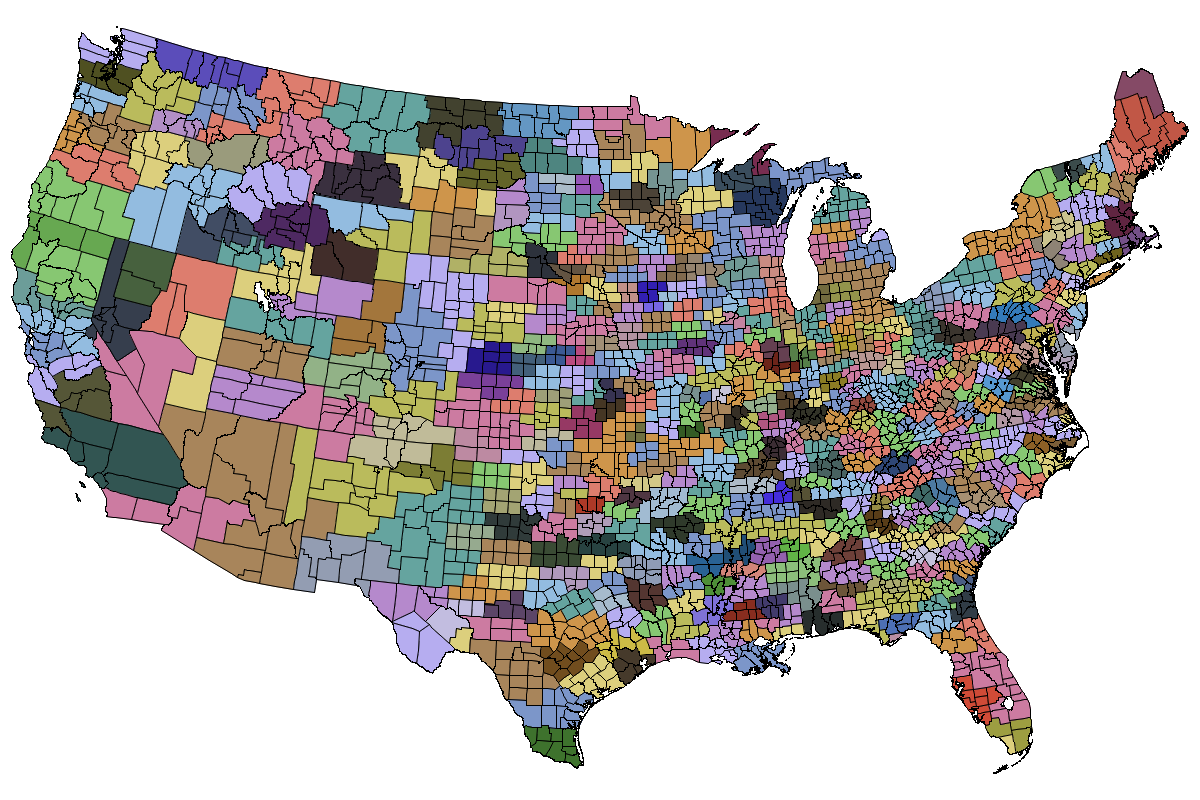
\includegraphics[width=.9\textwidth]{./figures/fastclus_map.png}
\label{fig:fastclusmap}
\end{figure}


%We graph the objective function value of this labor market definition in Figure \ref{fig:objfn_norm_fastclus}, labelled ``fastclus," comparing it with the other local labor market definitions. We find that while this definition initially does better than state, it is still less appropriate than 1990 and 2000 Commuting Zones. The likely cause is that our candidate areas are only selected based on geographic proximity; our next step is to include economic variables  such as wages and unemployment rates in the clustering method, which will \mc{likely improve our outcomes.}{ADF: Do we want a map of our resulting zones? Or will that not help? Or some quick summary statistics?} In theory, by minimizing the objective function, we should be able to arrive at a definition of labor markets that is at least as good as the Commuting Zone definition. Our ability to improve on the definitions will depend on developing improved methods for proposing candidate mappings of counties to clusters.

%\subsection{Spectral Clustering}



\subsection{Introduction to Spectral Clustering}

Spectral clustering classifies nodes by implementing k-means on the eigenvectors of a graph Laplacian of pairwise similarities \citep{vonLuxburg2007}. Spectral clustering can be explained as a random walk on the similarity graph, where the probability of jumping from one node to another is given by edge weights. In the stationary distribution of these stochastic jumps, a clustering may be thought of as the classification that minimizes jumps between clusters, for a given number of clusters. This interpretive framework is a natural way to think of local labor markets and job search or migration models. For this work, we assume an undirected or symmetric graph of similarities. Spectral clustering is a popular methodology implemented in a wide range of fields.

We implement normalized spectral clustering as defined by \cite{NgJordanWeiss2001}, which re-normalizes the rows of the eigenvectors for the number of clusters specified. This re-normalization has the advantage that even fairly isolated nodes end up clustered. In our experience, both hierarchical clustering and standard versions of spectral clustering were highly sensitive to the intensity of commuting flows and often failed to differentiate clusters outside of major urban centers. These residual, mostly rural, areas would end up lumped into a ``mega-cluster'' with little geographic integrity. Only by saturating the model with a high number of clusters (or a high threshold in the case of hierarchical clustering) could we allocate all counties to similarly sized clusters. With the methodology of \cite{NgJordanWeiss2001}, we can reliably allocate all counties to clusters for any quantity of clusters that we specify. We rely on the objective function to determine the optimal quantity of clusters, as implemented by normalized spectral clustering.

Spectral clustering is also amenable to classifying nodes based on multiple views of a graph, as we have argued is appropriate for characterizing local labor markets. Nodes may be characterized both by the intensity of pairwise links (.e.g commuting flows, distance, correlation of unemployment rates) and by feature space similarity (e.g. share employed in manufacturing). \cite{ZhouBurges2007} generalize single-view spectral clustering, showing that multi-views can be summarized in an undirected similarity graph as a weighted, linear combination of each view. Considering again the random walk interpretation of spectral clustering, \cite{ZhouBurges2007} interpret the multi-view graph as a mixture of Markov transition chains for each view. The objective function, which is also a linear combination of weighted values for each cluster, is not necessarily helpful for selecting an optimal weights. In the current implementation, we assign an equal linear weight to each view in the multi-view graph, using the same views that enter into the objective function. As with the objective function, the linear weights would depend on the economic interpretation of the clusters. 

The following, using notation from \cite{vonLuxburg2007}, describes the specific steps of our implementation of multi-view spectral clustering, with the goal of classifying $n$ counties into $k$ clusters:
\begin{enumerate}
   \item We construct an undirected similarity graph $S$, where the edge weights between nodes $i$ and $j$ are defined as $w_{ij}$, with the weight consisting of a linear combination of the set of views (e.g. commute flows, proximity, pairwise corrleation in unemployment rates).
   \item We compute the Laplacian, a symmetric matrix, as $L=Deg(S)^{-1/2}\cdot S \cdot Deg(S)^{-1/2}$, where $Deg(S)$ is the Degree matrix giving the row sums of $S$ on the diagonal.
   \item We compute eigenvalues and eigenvectors of $L$ and form an $n$ by $k$ matrix, $U$, from the $k$ eigenvectors with the largest eigenvalue.
   \item We form an $n$ by $k$ matrix $T$ by normalize the rows of $U$ to norm 1, each element $t_{ij}=u_{ij}/(\sum_{j \in k}u_{ik}^{2})^{1/2}$.
   \item We classify the $n$ rows of $T$ (one for each county) into $k$ clusters, $C_{1}, ... ,C_{k}$ using the k-means algorithm.
\end{enumerate}

\subsection{Implementation of Spectral Clustering}

In implementing this methodology, we use the similarity matrix implied by TS1996 as $S$, over which the Laplacian is computed. Additionally, in spectral clustering, the choice variable is not the cutoff height (as in hierarchical clustering) but the number of clusters, $k$. Rather than arbitrarily choose a number of clusters, we use our objective function specificed in equation \ref{eqn:objfn} to choose the set of clusters that is the most integrated, such that $k$ maximizes our objective function. Formally, we choose k such that:


\[
k*: ObjFn(C_{k*}) = \max\limits_{k \in [400,800]} ObjFn (C_k)
\]

Our resulting clusters are mapped in Figure \ref{fig:spectral}, and our calculations show that the optimal number of clusters is 656. Additionally, using our methodoogy clusters have an average of 4.74 counties each, which is larger than Tolbert and Sizer's defintions (4.24). Comparing Figure \ref{fig:spectral} with Tolbert and Sizer's commuting zones, there are a number of differences. First, our clusters are somewhat larger geographically. Second, the clusters in the East are larger in area than the clusters in Tolbert and Sizer's definitions. This is particularly telling in Florida, which has fewer clusters using our definitions. The same is true of Texas; in our clusters, the main metropolitan areas are visible, while they are not in Tolbert and Sizer. One notable similarity are the high frequency of very small clusters in Kansas. It appears that irrespective of methodology, there is not a lot of long-distance commuting in Kansas, which may reflect the different industrial composition.

\begin{figure}
\caption{Optimal Spectral Output, 656 Clusters\label{fig:spectral}}
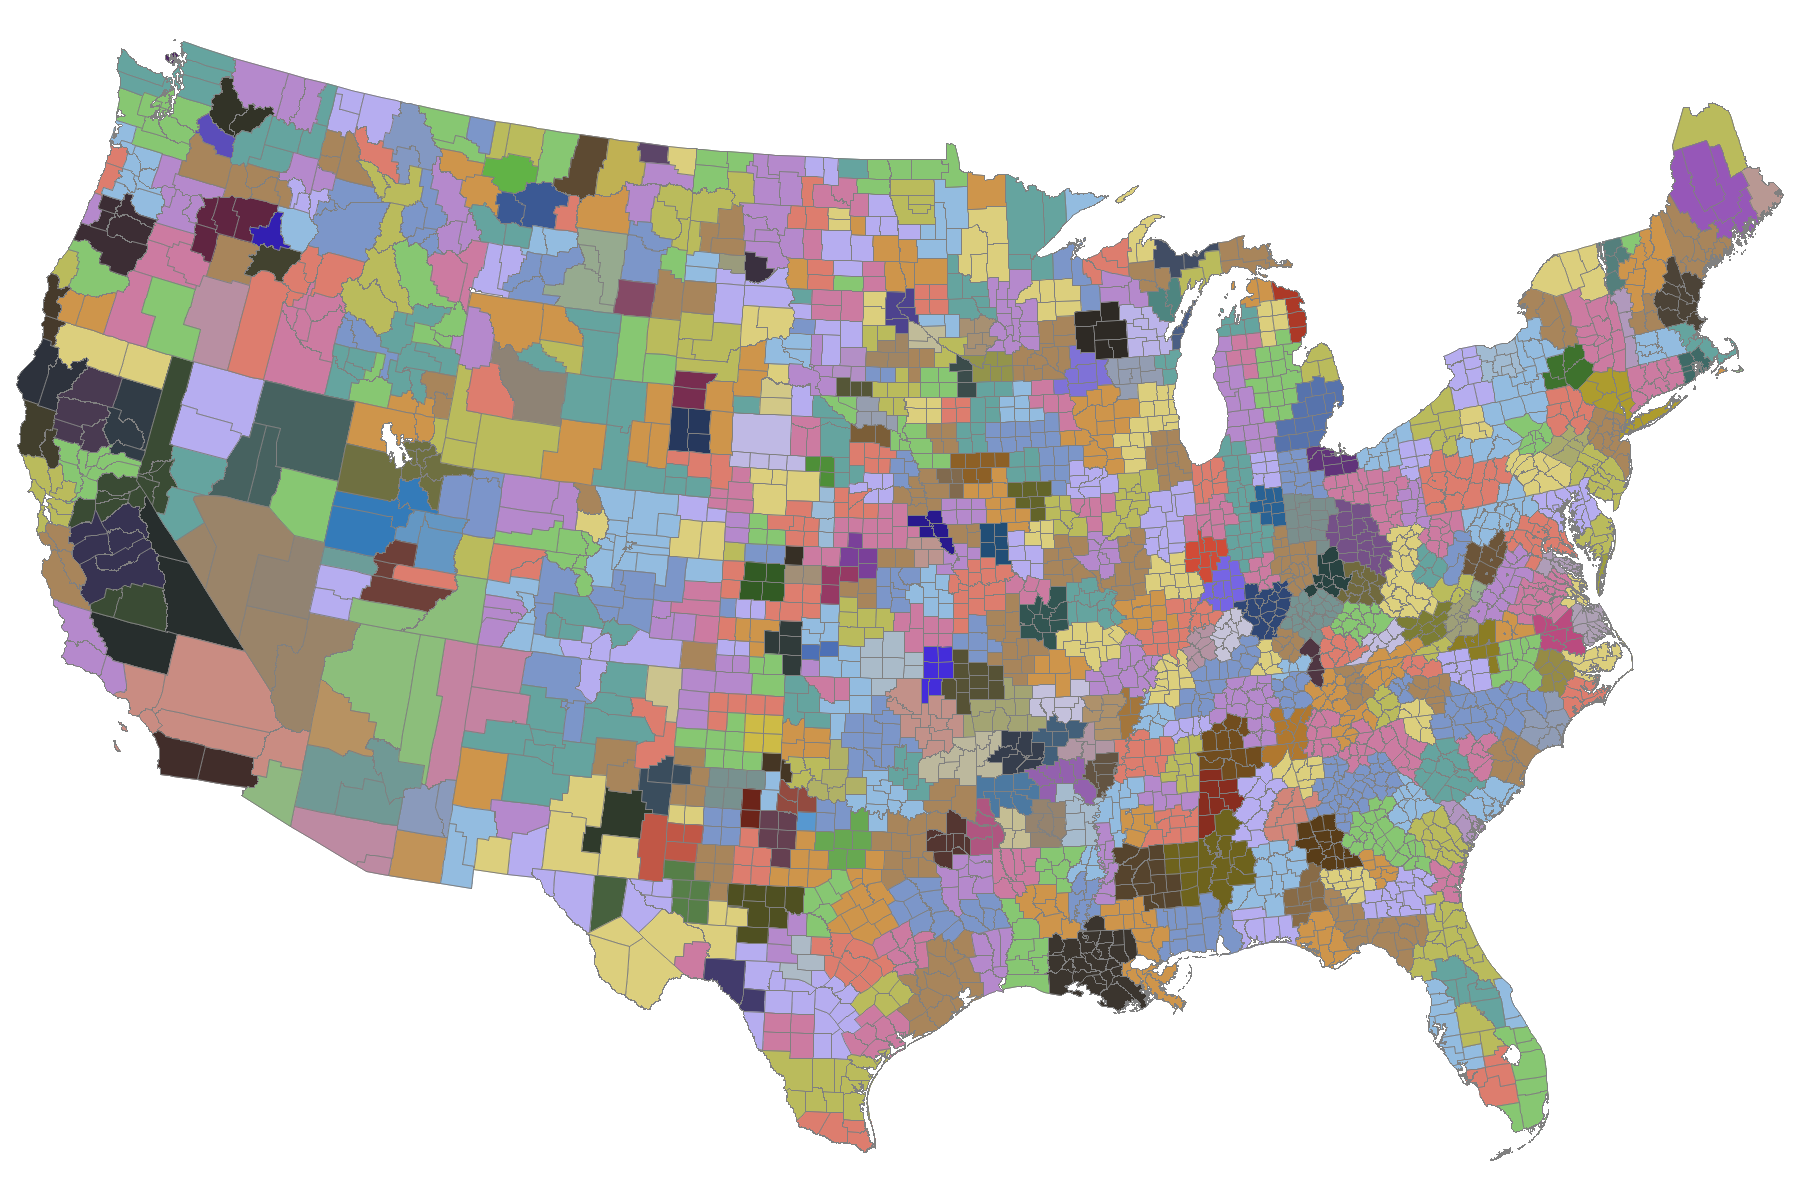
\includegraphics[scale=.4]{./figures/optimal_spectral_par.png}
\footnotesize \emph{Note:} Clusters are a result of authors' calculations, using methodology outlined in text.
\end{figure}

Next, we turn to comparing our results from the spectral clustering method with other local labor market definitions, using our objective function.

\subsection{Comparing Common Local Labor Market Definitions}

To compare our definitions to other candidate local labor markets, we calculate the objective function for a number of candidate local labor markets: our maximized spectral clustering definintion, Tolbert and Sizer's commuting zones, states, CBSAs (with a non-metro state residual), CBSAs only, and counties. These results are displayed in Figure \ref{fig:objfn_results}.

\begin{figure}\centering
\caption{Comparing Different Local Labor Market Definitions}
\begin{tabular}{c}
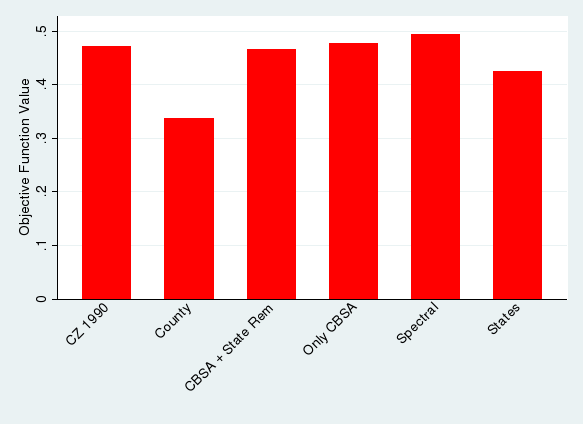
\includegraphics[scale=0.45]{./figures/objectivefunction_defns.png}\\
\multicolumn{1}{p{4.5in}}{\footnotesize \emph{Notes:} Author's calculations. CBSA definitions are 2010 current definitions. Data used in these calculations are discussed in Section \ref{sec:data}.}
\end{tabular}
\label{fig:objfn_results}
\end{figure}

Spectral clustering outperforms all other labor market definitions, while commuting zones are the next best option. If we use CBSAs and rest of state, our analysis shows that is somewhat on par with commuting zone definitions, while CBSA-only definitions only slightly outperform CBSA and state residuals. Finally, our analysis appears to suggest that counties are a poor representation of a local labor market compared with any other definition, even states.

In future work, we also want to compare these definitions over time, to see whether the decay in quality of local labor market definition is different across these definitions. This is especially relevant for current research which uses commuting zones, since these areas may not reflect current local labor market definitions.


%%%%%%%%%%%%%%%%%%%%%%%%%%%%%%%%%%%%%%%%%%%%%%

\section{Summary and Next Steps \label{sec:conclusion}}

Recent influential papers in labor economics have used commuting zones as an alternative definition to local labor markets. However, no one has carefully analyzed the methodology used to construct commuting zones and how it may impact empirical findings. Our paper contributes to this literature by analyzing this methodology and its implications for empirical applications.

We document that the commuting zone methodology is sensitive to uncertainty in the input data and parameter choices and we demonstrate how these features affect the resulting labor market definitions. Furthermore, we demonstrate that uncertainty in local labor market definitions also affects empirical estimates that use commuting zones as a unit of analysis. In future work, we want to explore other clustering methods, which are less history-dependent, as they may come to more globally optimal solutions. We also want to develop a measure with which to compare candidate zones against one another, using multiple metrics of local labor market integration.


	

%%%%%%%%%%%%%%%
% BIBLIOGRAPHY
%%%%%%%%%%%%%%%
\clearpage
\singlespacing

\bibliographystyle{aea}
\bibliography{bibliography}

\newpage
\appendix
\section*{Tables and Figures Appendix}
\FloatBarrier

\appendix
\setcounter{table}{0}
\renewcommand{\thetable}{A\arabic{table}}   
\setcounter{figure}{0}
\renewcommand{\thefigure}{A\arabic{figure}}   

\begin{figure}[th]
\caption{Various Height Cutoffs for California \label{fig:caliclusters}}
\begin{tabular}{cc}
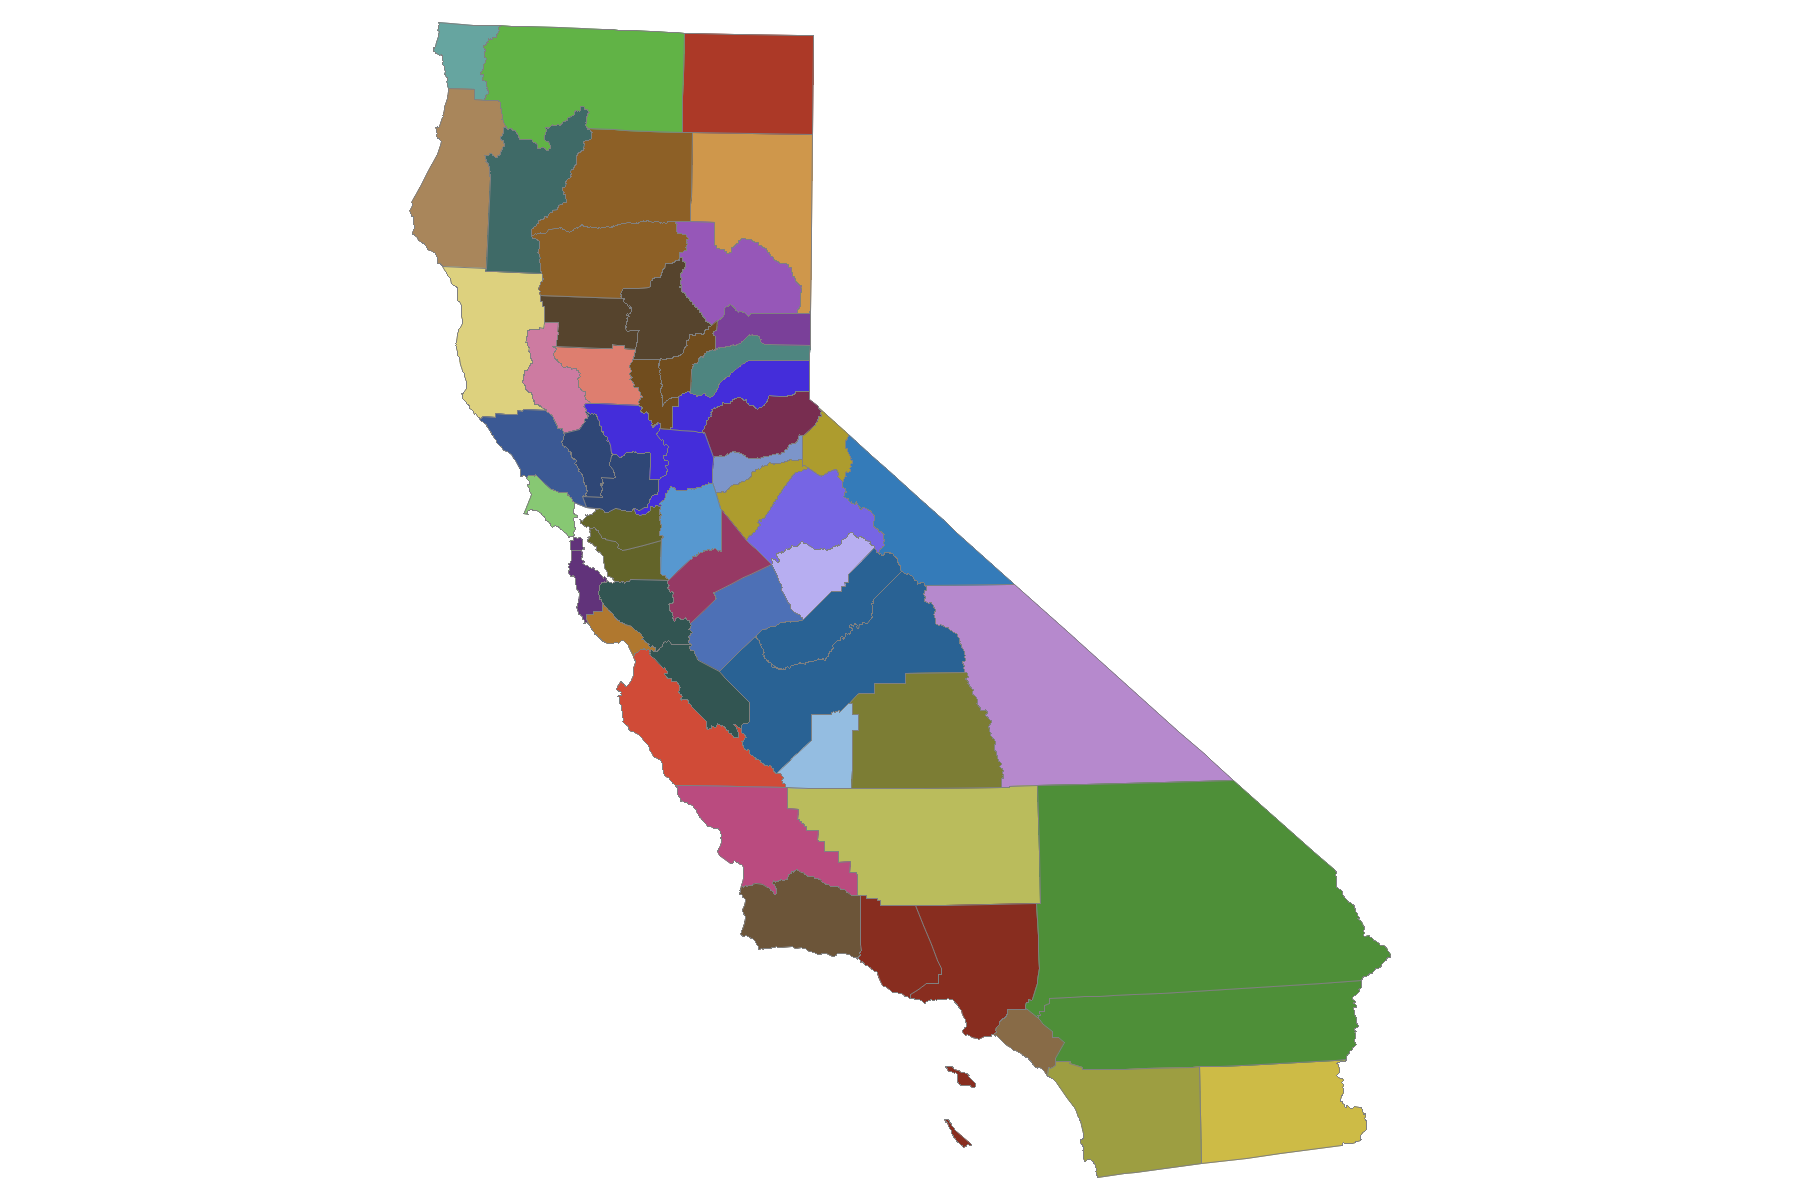
\includegraphics[scale=0.1]{./figures/insetmaps/california_clustermap_800_inset6.png} & 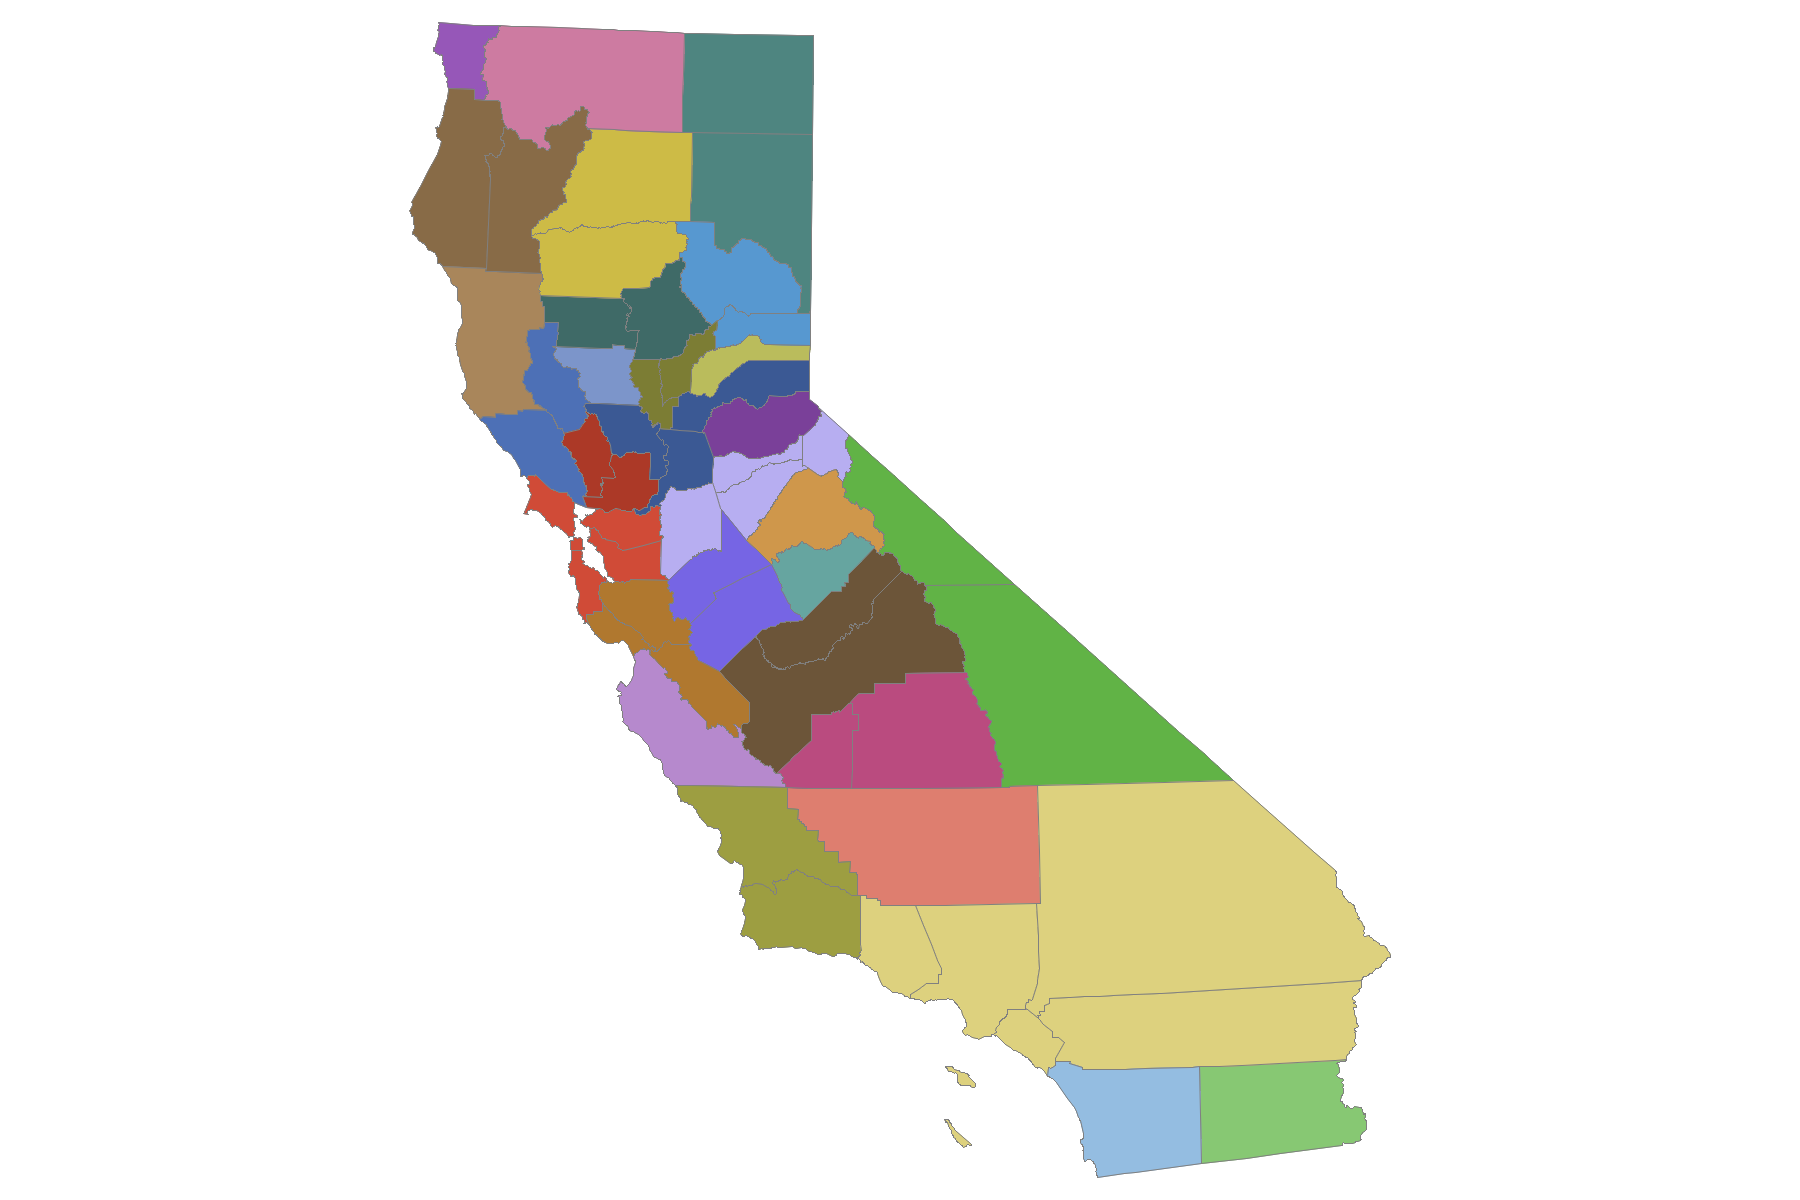
\includegraphics[scale=0.1]{./figures/insetmaps/california_clustermap_880_inset6.png} \\
Height = 0.8 & Height = 0.88 \\
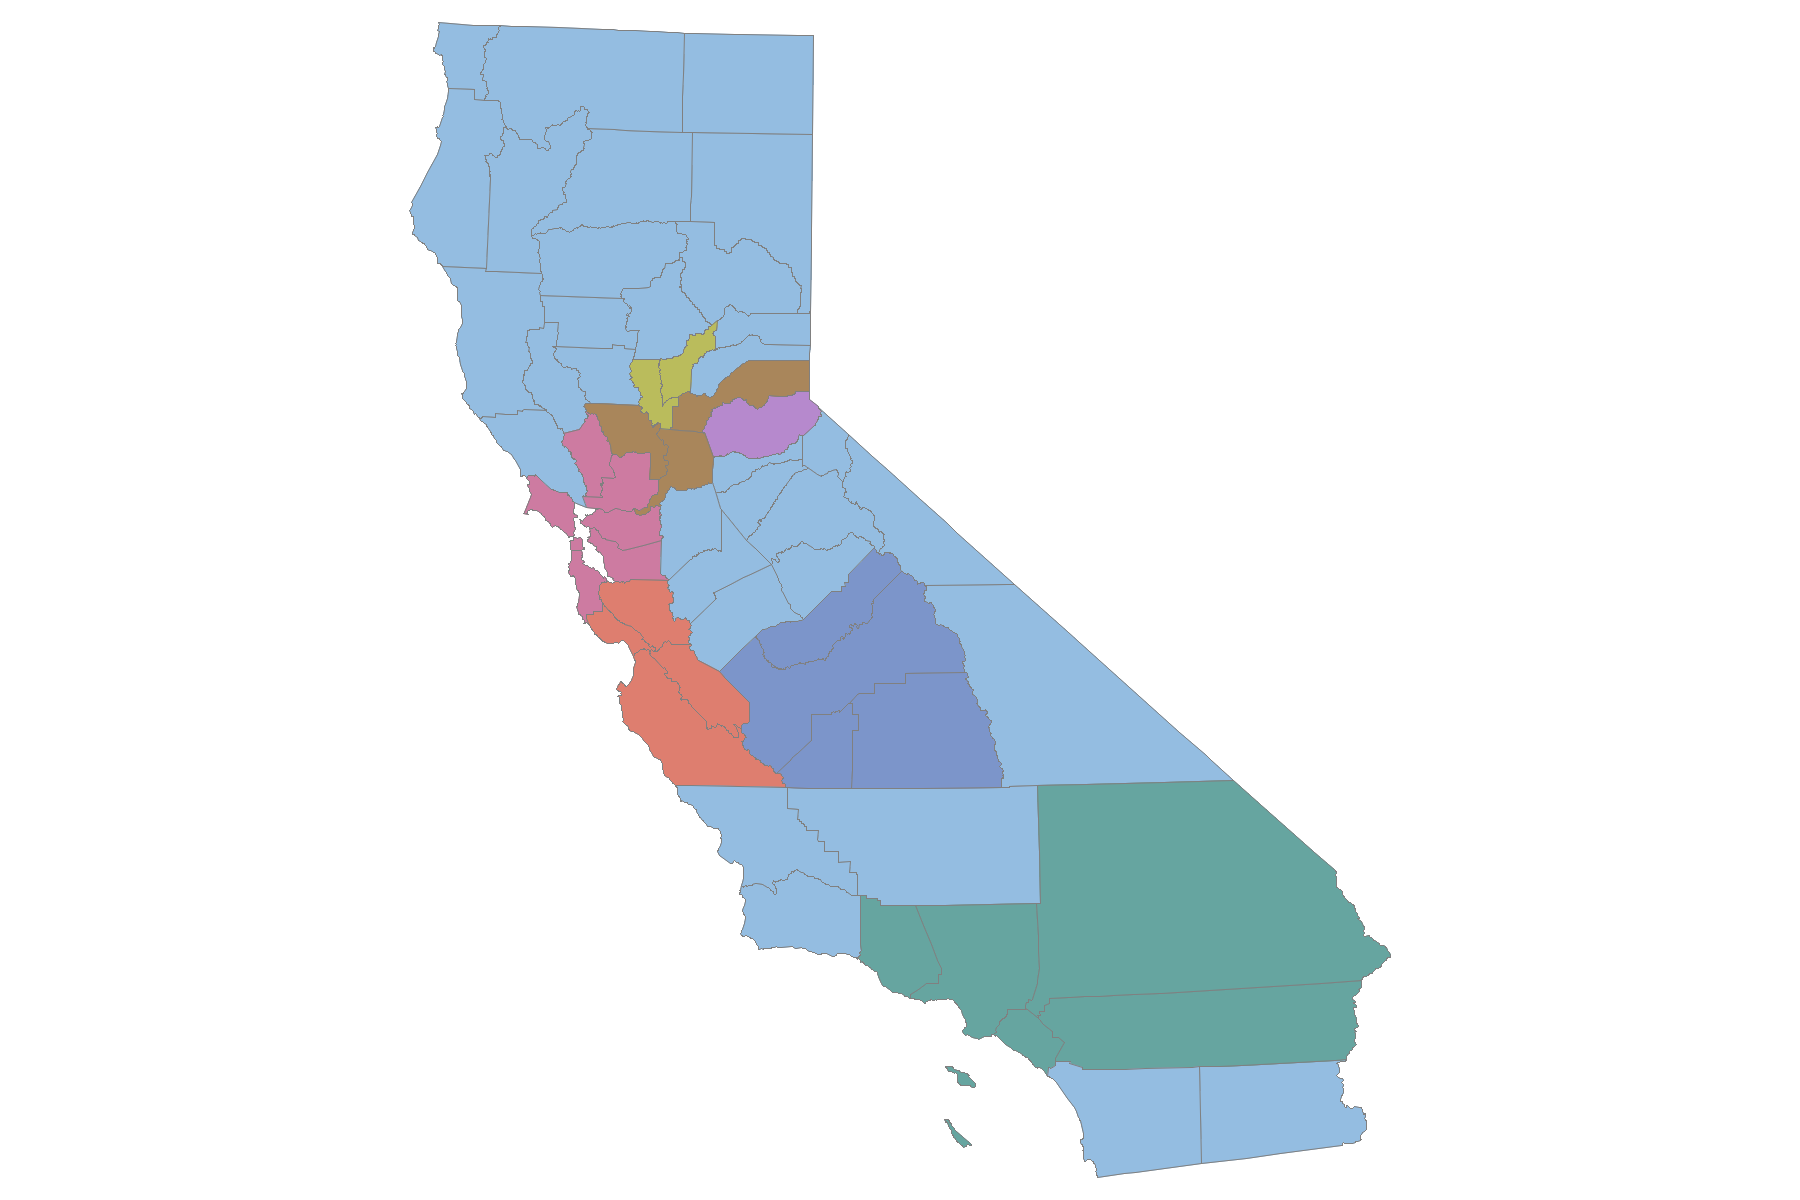
\includegraphics[scale=0.1]{./figures/insetmaps/california_clustermap_960_inset6.png} & 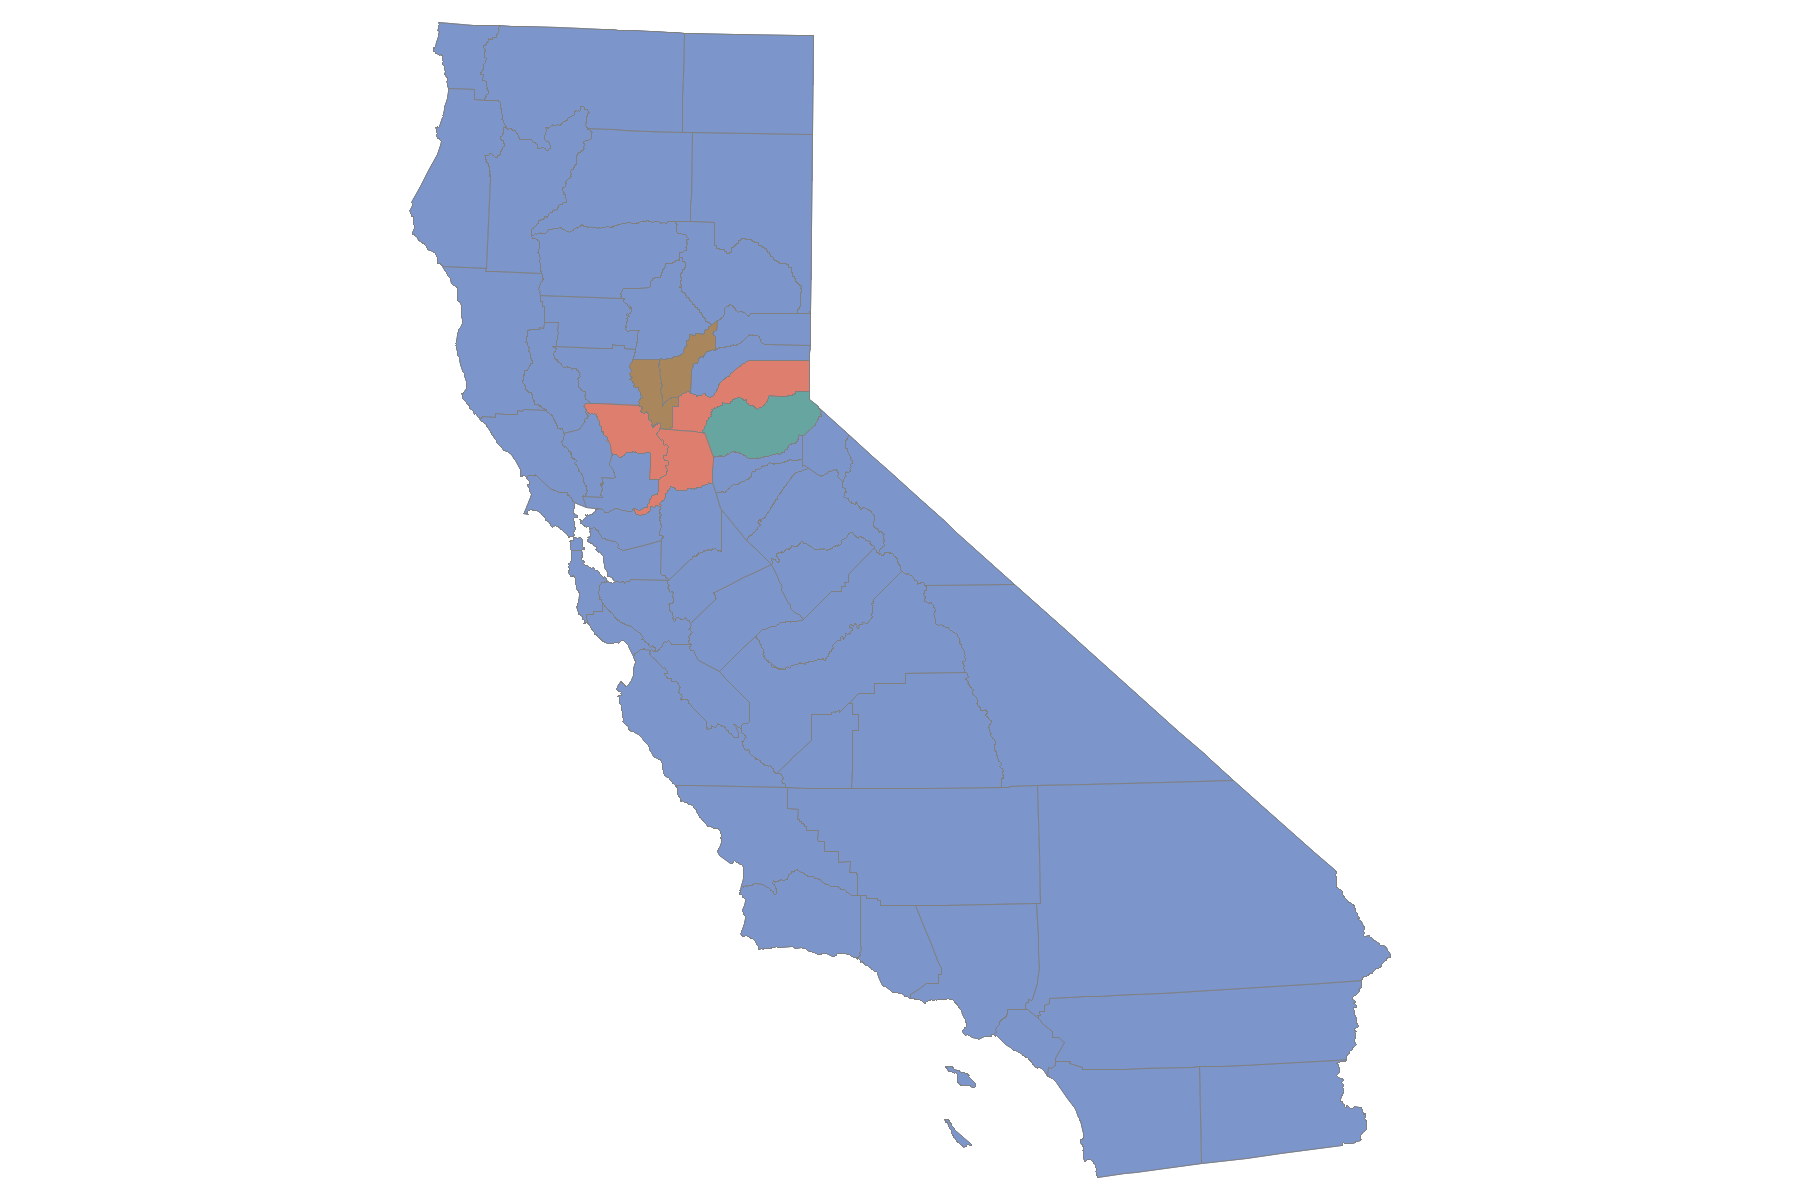
\includegraphics[scale=0.1]{./figures/insetmaps/california_clustermap_1000_inset6.png} \\
Height = 0.96 & Height = 1\\
\multicolumn{2}{p{5in}}{\footnotesize \emph{Notes:} The above graphs are generated using the methodology outlined in Section \ref{sec:method}, using 1990 Census JTW data. More detail is in the text.}
\end{tabular}
\end{figure}

\begin{table}[h]
\caption{Summary Statistics of Ratio of MOE to Flows \label{tab:moesum}}
\begin{tabular}{lcccc}
\hline\hline
& Mean & 25th Pctile & 50th Pctile & 75th Pctile \\
\hline
All counties & 1.236 & 0.845 & 1.370 & 1.600\\
Flows <100 & 1.432 & 1.148 & 1.500 & 1.636 \\
Flows 100-1000 & 0.444 & 0.301 & 0.414 & 0.549  \\
Flows 1000-10000 & 0.131 & 0.087 & 0.124 & 0.169 \\
Flows 10000+ & 0.037 & 0.024 & 0.036 & 0.049 \\
\hline\hline
\multicolumn{5}{p{4in}}{\footnotesize \emph{Notes:} Author's calculation using
2009-2013 ACS Journey-to-Work data.}
\end{tabular}
\end{table}






\end{document}
